% !Mode:: "TeX:UTF-8"

\chapter{分层光网络下的并行路由优化算法研究}
\section{引言}
  随着视频流、云计算服务和移动应用的普及,互联网的流量不断增加[],业务量的持续增长给互联网的传输带来了巨大的挑战,为了满足日益增长的容量要求,波分复用(WDM)系统已部署在骨干网络,其每个通道带宽高达40 GB/s或100 Gb/s。现在,400 Gb/s的带宽接口已经在实验室[2]实现,此外,为了满足不同的数据速率服务异构的流量类型,混合线路速率(10/40/100Gb/s)的WDM系统也已经部署。因此,WDM光网络视乎为大流量业务传输提供了一个既实际又高效的解决方案。
  然而,传统的WDM光网络严格遵循ITU-T的固定均匀间距和网格(通常为50)GHz或100千兆赫)[],这样会导致低效的频谱利用率,比如,一个较大的波长可能会被分配给一个低速率的业务,即使这个业务根本就不能占满整个波长。很明显,传统WDM光网络的不灵活和粗粒度的带宽控制会导致显著的频谱浪费,限制了提高其网络容量的潜力。
  为了应对WDM网络的低敏捷性和频谱浪费问题,近年来,弹性光网络(EON)的架构被提出,在EON架构中,存在细粒度的带宽间隙(比如,12.5GHZ),他比WDM网络所遵循的ITU标志的50GHZ或者100GHZ的带宽粒度要小很多,而且,这些带宽间隙可以根据需要被组合在一起以提供更宽的通道。所以为了提高带宽利用率,在EON中存在混合速率,每个速率的业务需要不同数量的频谱间隙数量。理论上,EONs能够灵活地提供各种速率,但是在实际中,EONs却可能只含有很少的速率种类,这主要是因为:第一,随着频谱的增加,频谱碎片和管理复杂度将显著增加。第二,实际的EON从较低的线路费率升级到更高的线路费率,并存大量速率的情况已经很少见了。
  为了在EON网络中加入业务,控制平面必须在网络中找到一条路径,同时,还需要在此路径上的链路上分配足够的频谱带宽,来创建一个合适的端到端光路连接,这被称为路由和频谱分配(RSA)问题,EONs中的RSA问题比传统的在WDM网络中的路由和波长分配(RWA)问题更具有挑战性,传统的RWA解决方案[][]在EONs中已经变得不再适应了。在EONs中一个业务需求可能需要多个连续的频谱间隙,而且由于缺少全光谱转换器,每条光连接的频谱从它的源节点到它的目的节点 ,在所经过的链路上保持不变,这被称为频谱连续性限制。
  根据流量模式,RSA问题可以进一步分为静态RSA问题和动态RSA问题。静态的RSA问题出现在网络规划阶段,其中流量需求是已知的,这样可以离线计算出最优或者接近最优的RSA解,动态RSA问题是指在实时业务情况下光通路的路由选择和波长分配的优化问题,在动态RSA问题中,业务随机的到达和离开光网络,而且当业务到达网络时,控制平面需要在短时间内找到RSA解来安排业务。动态RSA问题比静态RSA问题更具有挑战性,因为业务需求随机到达和离开,网络状况随时发生变化,而且要求控制平面反应实时。
 链路代价表示路由路径选择这一条链路所需要的代价,链路代价可以设置为链路的距离,延迟,租用链路需要的费用等等,业务的路由代价表示业务路径经过的链路的代价总和,路由代价反应了路由路径的优劣程度,如果链路代价设置为延迟,则路由代价越小表示路由整体延迟较小,如果链路代价设置为1,则路由代价越小,表示路径经过的跳数越小,使用的链路资源越小。
 本章考虑在EONs中解决动态RSA问题,设计出带跳限约束下的基于分层图的动态路由优化算法来优化整体路由代价,分别考虑无权图和带权图上的算法GPU加速设计,GPU并行版本达到平均近6倍的算法加速比,实验与分层图上的传统算法比较,显示该算法过程在短时间内能够大量的优化路由代价,并且由于路由选择较优,使用网络资源较少,最终网络阻塞率表现也有显著的提高,实现了快速的路由代价优化和整体的阻塞避免。
\section{问题描述}
\subsection{EONs中动态RSA问题}
  在动态场景中,业务的到达时间和服务时间都是随机的,当业务到达网络时,SDN控制层需要找到可行的路径,并且为路径分配合适的频谱资源。由于EON的物理限制,RSA问题的解需要满足以下限制:
%\begin{enumerate}[(i)]
第一,传输距离限制:光信号的传输质量会随着传输距离的增加而下降,为了在目的点顺利恢复光信号,光链路的传输距离需要小于一个阈值$D_max$,为了简化设计,本文假设每一条链路的长度相同,都是一个单位,那么传输路径的跳数需要小于阈值$D_max$。
第二,频谱连续性限制:每条光连接的频谱从它的源节点到它的目的节点 ,在所经过的链路上保持不变。
第三,频谱不重叠限制:同一光纤链路中的频谱不能分配给不同的光路。
第四,频谱邻近限制:频谱邻近约束保证分配给一个光路径的频谱必须是一个连续的部分。
 此外,为了限制路径对网络频谱的资源使用,我们为路径加入跳限约束,论文[]中对网络加入跳限约束,使得整体上阻塞率降低,此外,后面将讨论,加入跳限约束后能够简化GPU上代码的实现,使得算法可以提前结束,节省同步标记。
\subsection{分层网络模型}
  论文[]中提出一种分层图模型来解决WDM网络中的路由和波长分配问题,分层图模型将路由选择和波长分配问题统一到一起来,使得RWA问题变得简化,这种分层图模型也可以很容易推广到EONs的RSA问题中。
  我们使用有向图$N(V,E)$表示物理网络拓扑,其中$V={v_1,v_2,...,v_N}$表示节点集合,$E={e_1,e_2,e_3,...,e_M}$表示边集合,$e_k=(i_k,j_k)$表示边的头节点为$v_{i_k}$,边的尾节点为$v_{j_k}$。假设所有光链路具有相同的频谱范围$W=(F_{start},F_{end})$,其中$F_{end}-F_{start}=C$。EON所支持的速率集合为$R$,比如,$R={40Gb/s,100Gb/s,400Gb/s}$,每一种速率$r\in R$需要一个特定的频谱宽度$b_r GHz$。一个源节点为$s$,目的节点为$t$,速率为$r Gb/s$的业务被表示为$TD(s,t,r)$。
  下面我们讨论分层图的产生过程,假设第一个速率的为$r$的业务$TD_r(s,t)$到达网络,我们从可用的频谱切割出一块频谱大小为$b_r$的连续带宽分配给速率为$r$的业务,假设这块频谱的起始频率为$fs_{(r,1)}$,终止频谱为$fe_{(r,1)}$,那么$fe_{(r,1)}-fs_{(r,1)}=b_r$,我们把所有物理链路上频谱范围$(fs_{(r,1)},fe_{(r,1)})$,从链路上“割”下来,把“割”下来的部分组成一个新的虚拟网络$N^{(r,1)} (V^{(r,1)},E^{(r,1)})$,在这个新的网络中每条链路的频谱范围都是$(fs_{(r,1)},fe_{(r,1)})$,这样切割下来之后,原来的物理网络的频谱范围更新为$(F_{start}+b_r,F_{end})$。
  然后在这个复制出来的图上为业务求一条最短路径$p$,那么容易知道路径$p$一定满足约束2,3,4,这样问题被简化为单纯的路由问题。要注意的是,这个虚拟图上频谱不能再分配给其他速率为$r'$的业务$TD_r'(s',t')$,即使$b_r'<b_r$,这是因为这样会产生大量的频谱碎片,使得频谱利用率下降,阻塞率降低,并且这样会使得问题变得更加复杂化,所以这些分割出来给速率$r$的频谱,将继续被分配给速率为$r$的业务。当下一个速率为$r$的业务$TD_r (s'',t'')$到达网络后,他首先在图$N^{ (r,1)}(V^{(r,1)},E^{(r,1)})$中寻找路径,如果找到合适的路径则加入网络并且更新路径链路的可用频谱为0;反之,如果他在图$N^{(r,1)} (V^{(r,1)},E^{(r,1)})$中没有找到合适的路径,那么算法会重新去”切割“物理拓扑得到虚拟网络$N^{(r,2)} (V^{(r,2)},E^{(r,2)})$,这样随着大量业务的动态的到达和离去,会产生大量的虚拟图,频谱资源已经大量地分布在各个虚拟图中,我们把这些虚拟图叫做分层图(layered Graph),现在RSA问题转化为在分层图中求解路由的问题,问题被简化。
  下图表示分层图示意,原图被切割成一个分层图集集合$L$,$L_i \in L$表示速率$i$的分层图集,如图所示,速率$k$的一共有$|L_k|$个图副本,每个子分层图占用频谱$(fs_{(r,1)},fe_{(r,1)})$,图中,点$v_i^{(r,l)}$表示速率$r$的第$l$层图上的第$i$号点。
$f_{()}$
\begin{figure*}
\setlength{\belowcaptionskip}{-0.5cm}
  \begin{center}
    {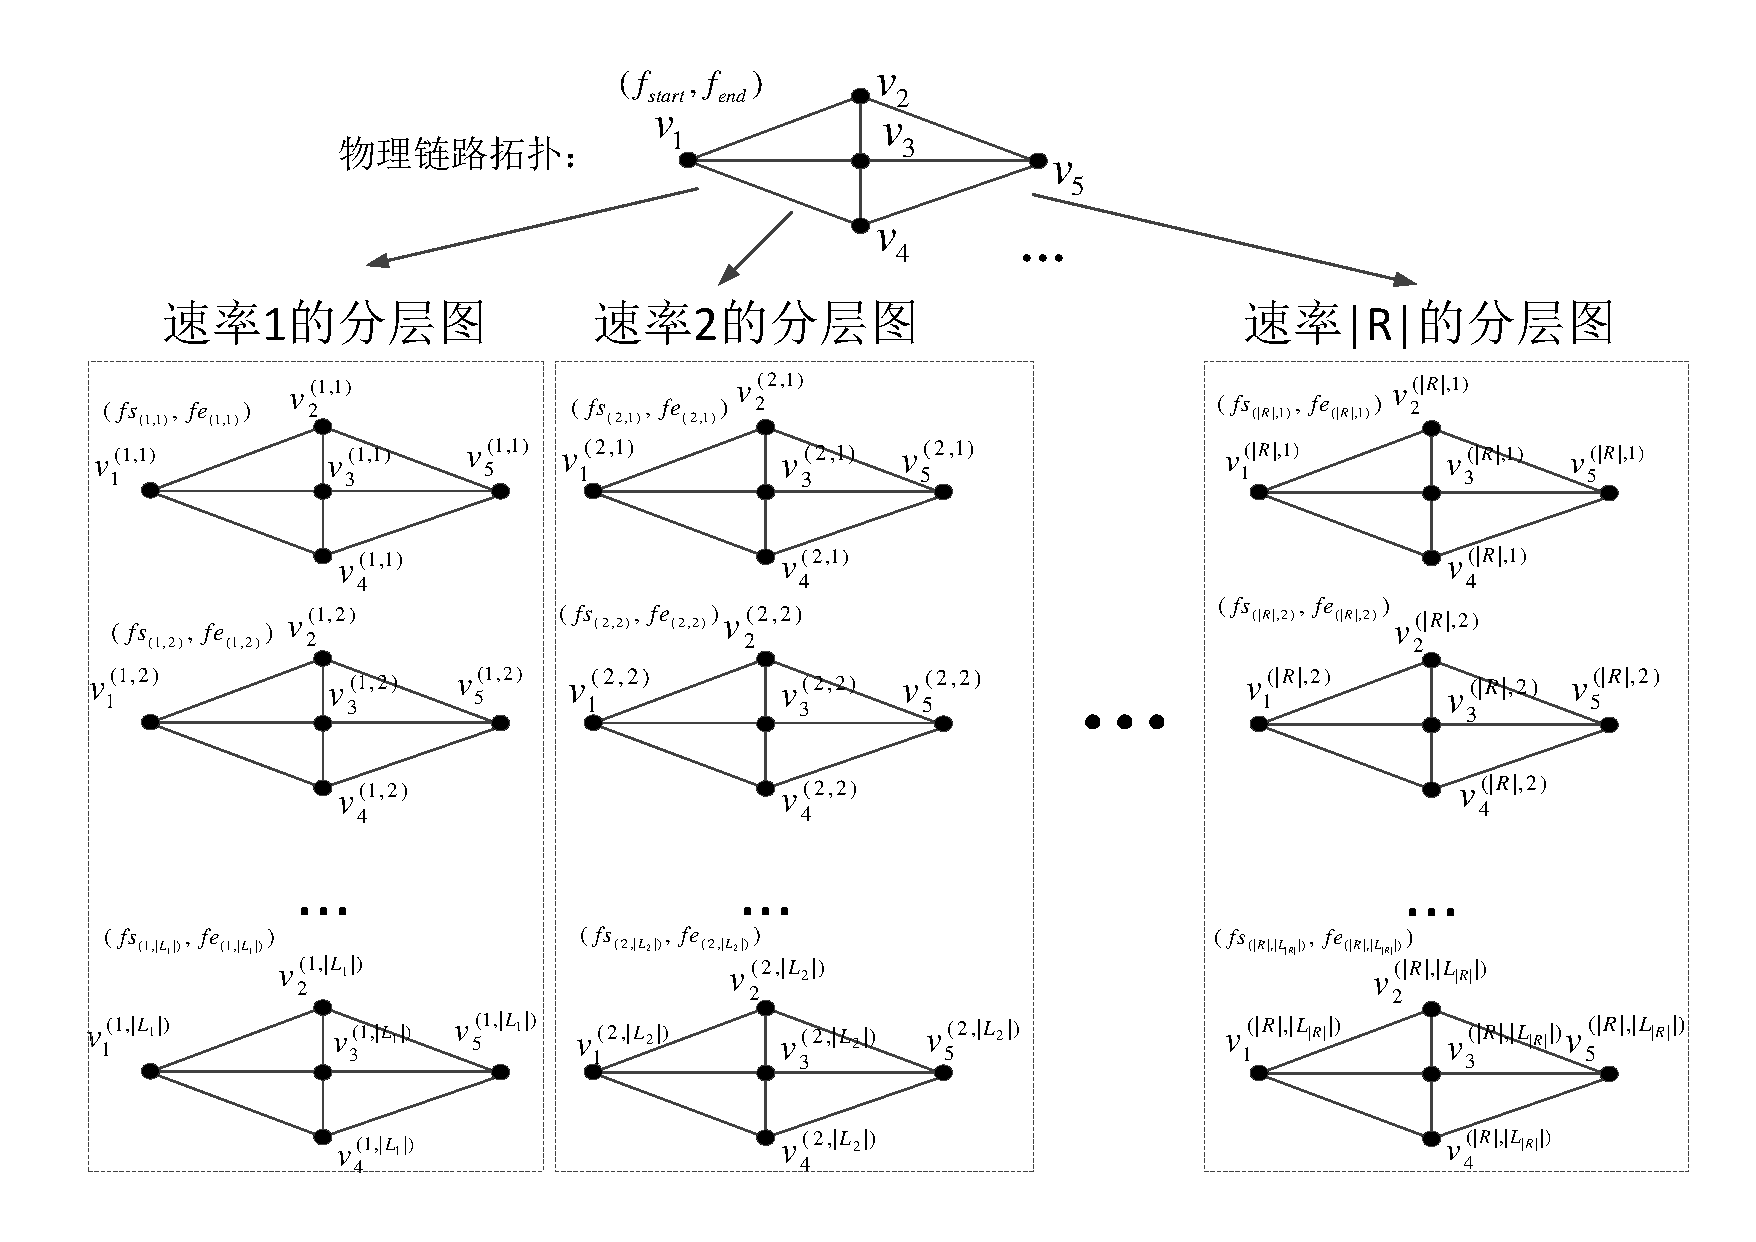
\includegraphics[width=1 \textwidth]{figures/LAYER.pdf}}
    \end{center}
  \caption{{\footnotesize{分层图示意}}}
  \label{layer}
\end{figure*}
\section{主要优化流程}
  根据前面的讨论,当一个速率为$r$的业务$TD_r(s,t)$到达网络时,一共有$L_r$个分层平面都可以用于此业务,也就是说如果在这些图当中都能为业务找到合适的路径的话,那么业务就有$L_r$条路径可供选择,我们可以选择代价最小的一条来优化路由。进一步,当有一批速率为$r$的业务集合$TD_r$到达网络时,如果大家都选择同一层加入的话,会出现大量的冲突,而且路由代价也会很大,但是由于现在有多个分层图平面可以选择,每个业务都有$L_r$条路径可以选择,这就给路由优化提供了可能,不同的业务需求可以选择不同层上的路径来进行路由,以使得总体路由代价减小,节省网络频谱资源,从而优化阻塞率。本节提出一个基于分层图的动态RSA优化算法流程,算法流程图如下所示:
 \begin{figure*}
\setlength{\belowcaptionskip}{-0.5cm}
  \begin{center}
    {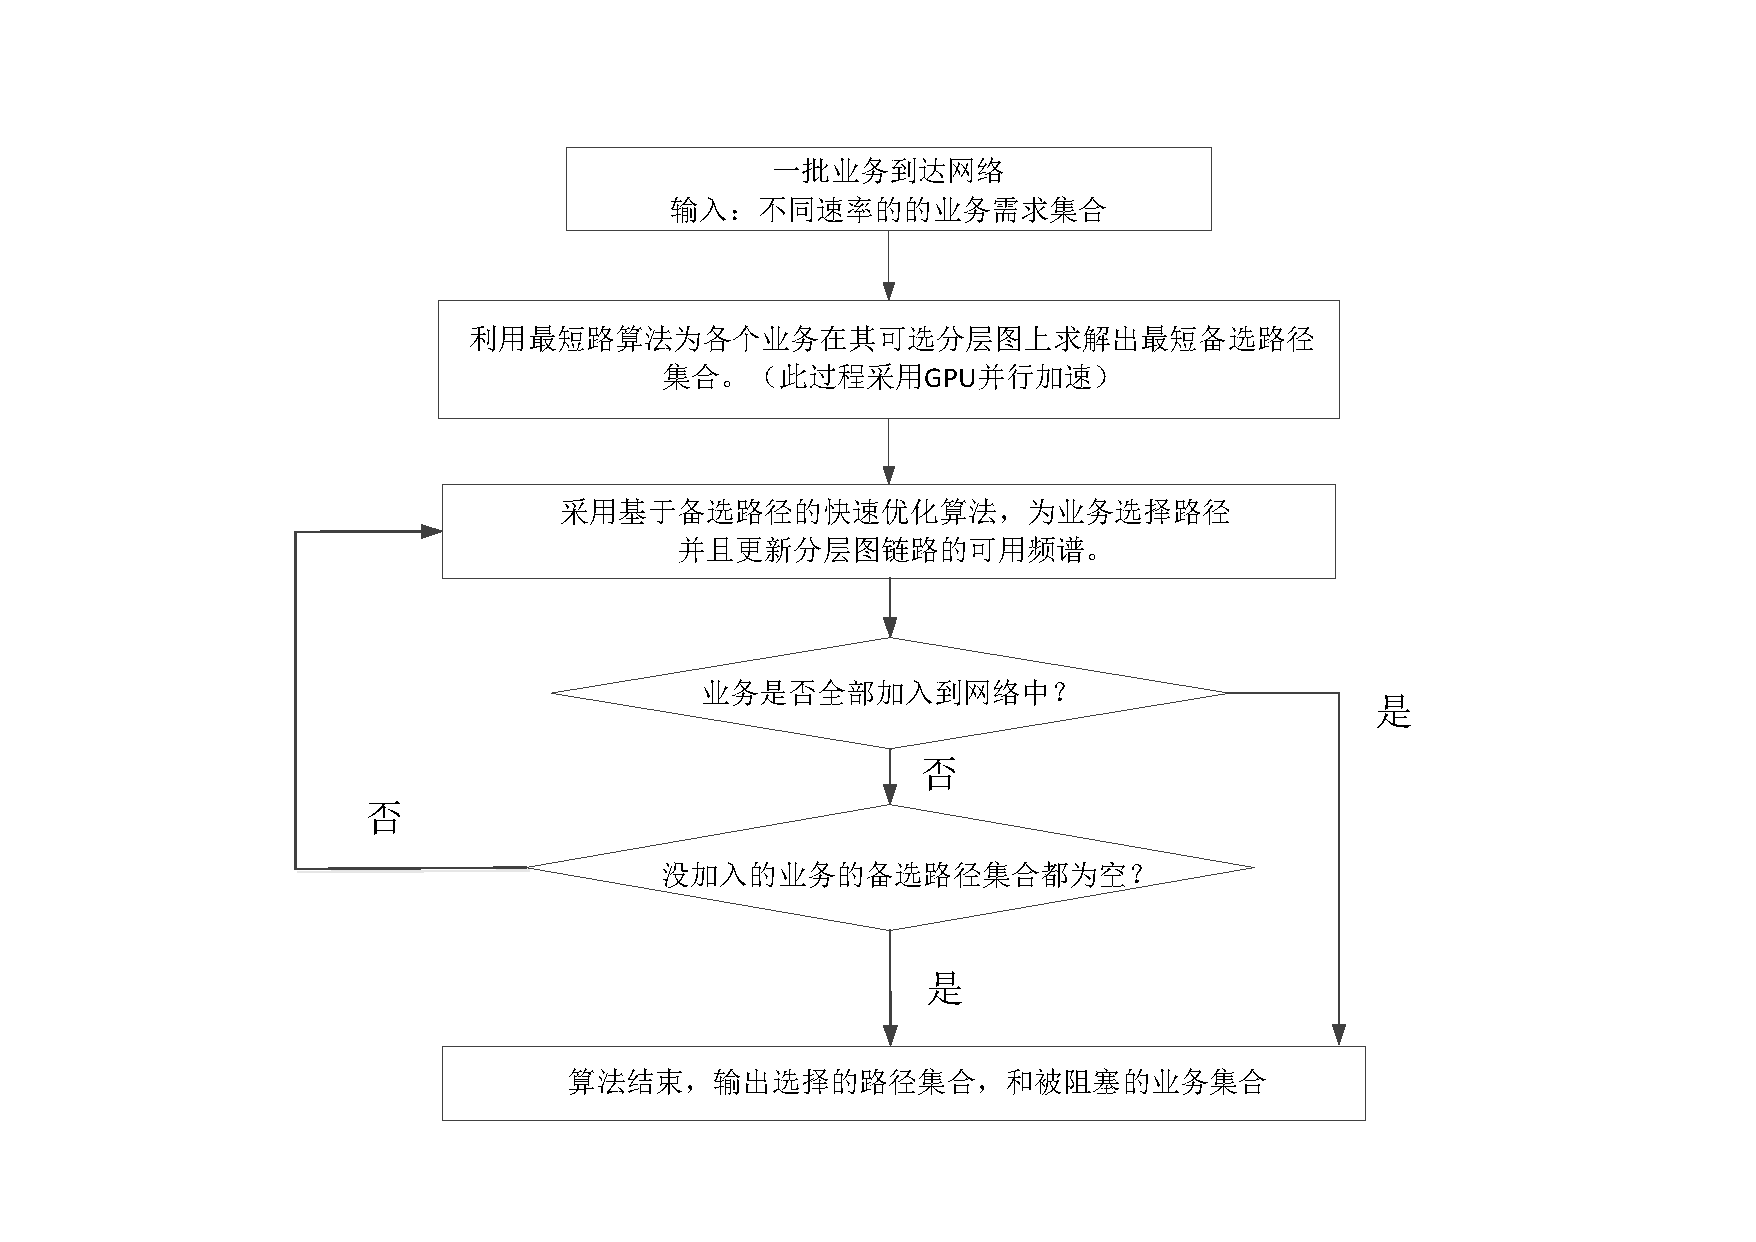
\includegraphics[width=1 \textwidth]{figures/bbprocess.pdf}}
    \end{center}
  \caption{{\footnotesize{算法优化流程}}}
  \label{bblayer}
\end{figure*}
\section{无权图情况下的GPU算法设计}
\section{带权图情况下的GPU算法设计}
\section{实验仿真分析}